\documentclass[11pt,a4paper]{article}
\usepackage[margin=22mm]{geometry}
\usepackage{amsmath}
\usepackage{booktabs}
\usepackage{graphicx}
\usepackage{float}
\graphicspath{{figures/}}
\setlength{\parindent}{0pt}
\setlength{\parskip}{5pt}
\renewcommand{\arraystretch}{1.22}

\setlength{\textfloatsep}{10pt}
\setlength{\intextsep}{10pt}

\begin{document}

\begin{titlepage}
\centering
\vspace*{2cm}
{\Large\textbf{ASSIGNMENT REPORT-6}}\\[0.7cm]
{\large\textbf{GAUSSIAN MIXTURES AND K-MEANS CLASSIFICATION}}\\[1.7cm]
\textbf{Submitted by:}\\[0.4cm]
\textbf{KARTHIKEYAN M} [26120004]\\[0.3cm]
\textbf{MIRTHULA M} [261200121]\\[1.8cm]
\textbf{Under the guidance of:}\\[0.4cm]
\textbf{HEMA ARUNACHALAM MURTHY}\\[1.5cm]
\textbf{For the subject}\\[0.4cm]
{\Large\textbf{Pattern Recognition and Machine Learning}}\\[0.3cm]
\textbf{(26AI5707)}
\vspace{2cm}

{\textbf{DEPARTMENT OF COMPUTER SCIENCE \& ENGINEERING}\\[0.3cm]
\textbf{SHIV NADAR UNIVERSITY, CHENNAI}\\[0.3cm]
\textbf{OCTOBER 2026}}
\end{titlepage}

\section*{INTRODUCTION}

This experiment is all about working with Gaussian Mixture Models and K-Means Clustering. We generate 2 Gaussian Mixtures that denotes the two classes we would be working on.

\section*{EXPERIMENTAL SETUP}
\begin{center}
\small
\begin{tabular}{llll}
\toprule
Classes & 2 & Gaussian components per class & 3 \\
Samples per class & 5,000 & Mixture weights & $(0.5,\,0.3,\,0.2)$ \\
Training / testing per class & 4,000 / 1,000 (80--20) & K-means centres per class & 3 \\
Convergence tolerance & $10^{-6}$ & Maximum iterations & 100 \\
\bottomrule
\end{tabular}
\end{center}

\begin{center}
\small
\setlength{\tabcolsep}{5pt}
\begin{tabular}{ccccc}
\toprule
Component & Class 1 mean & Class 2 mean & Class 1 covariance & Class 2 covariance \\
\midrule
Bottom & $(-1,-3.5)$ & $(6,-3.5)$ &
$\begin{bmatrix}1&0.6\\0.6&1\end{bmatrix}$ &
$\begin{bmatrix}1&-0.6\\-0.6&1\end{bmatrix}$ \\[9pt]
Middle & $(0,0)$ & $(7,0)$ & $\begin{bmatrix}1&0\\0&1\end{bmatrix}$ & $\begin{bmatrix}1&0\\0&1\end{bmatrix}$ \\[9pt]
Top & $(1,3.5)$ & $(8,3.5)$ &
$\begin{bmatrix}1.5&0\\0&0.5\end{bmatrix}$ &
$\begin{bmatrix}1.5&-0.5\\-0.5&0.5\end{bmatrix}$ \\
\bottomrule
\end{tabular}
\end{center}

\section*{GAUSSIAN MIXTURE DATA}

Here the left side 3 gaussian components belong to class 1 and right side 3 belongs to class 2. Also, when we are generating the gaussian mixture we use some weights to determine how much weightage each component gets. For eg. In our class we has $0.5$ for the bottom most component and hence, they get about approximately $2,500$ points out of $5,000$ points that were generated.

\begin{figure}[H]
\centering
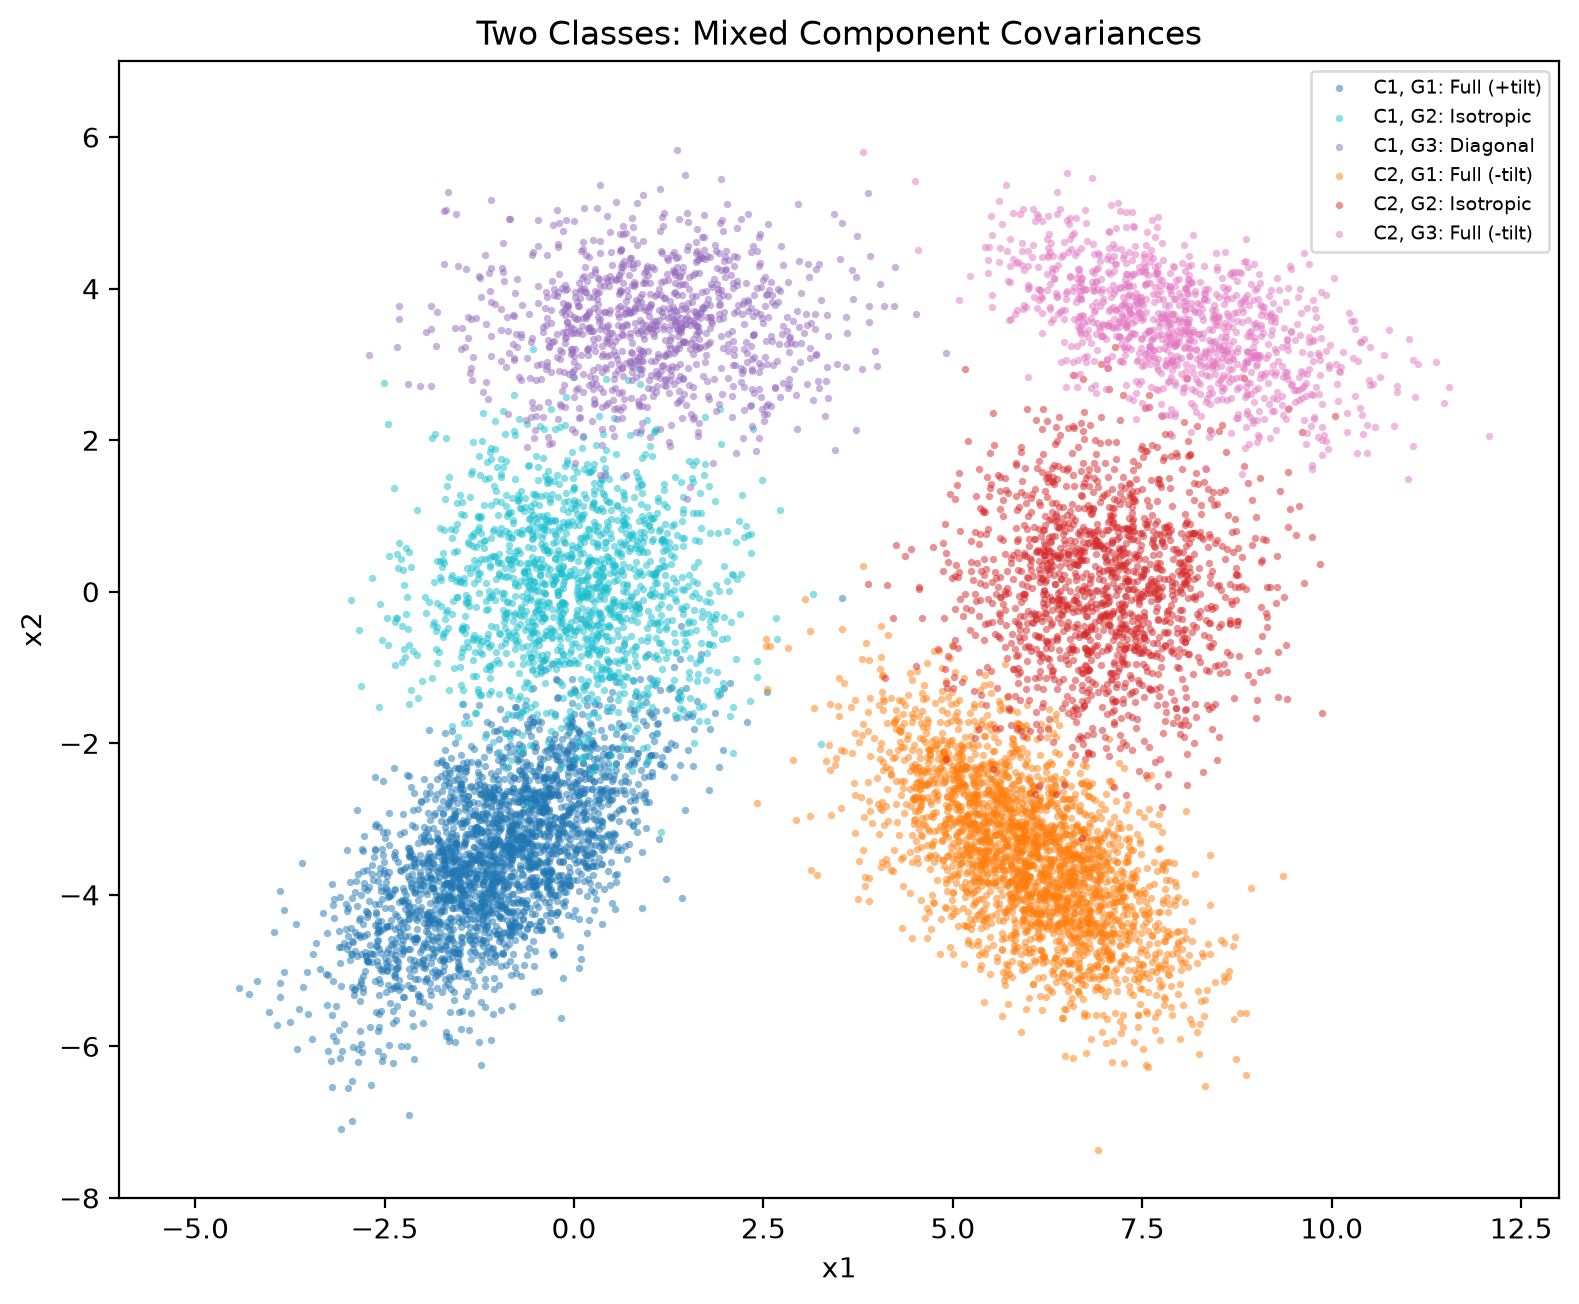
\includegraphics[width=0.70\textwidth]{mixture_data.png}
\caption{Two classes, each generated from three Gaussian components.}
\end{figure}

\section*{WITHIN-CLASS K-MEANS CLUSTERING}

So, here we do K-Means clustering for each of those 2 classes. We do a 80-20 split, and we cluster with the $80$ percentage of the training data and hold out the 20 for testing. We start with randomly initializing the centroids and assign each point to the nearest centroids and then recalculate the mean and have them as new centroids and repeat the same process until convergence or 100 iterations. Here we use squared euclidean as the distance measure. The decision boundary is drawn where you have equal distance measure between multiple centroids.

\begin{figure}[H]
\centering
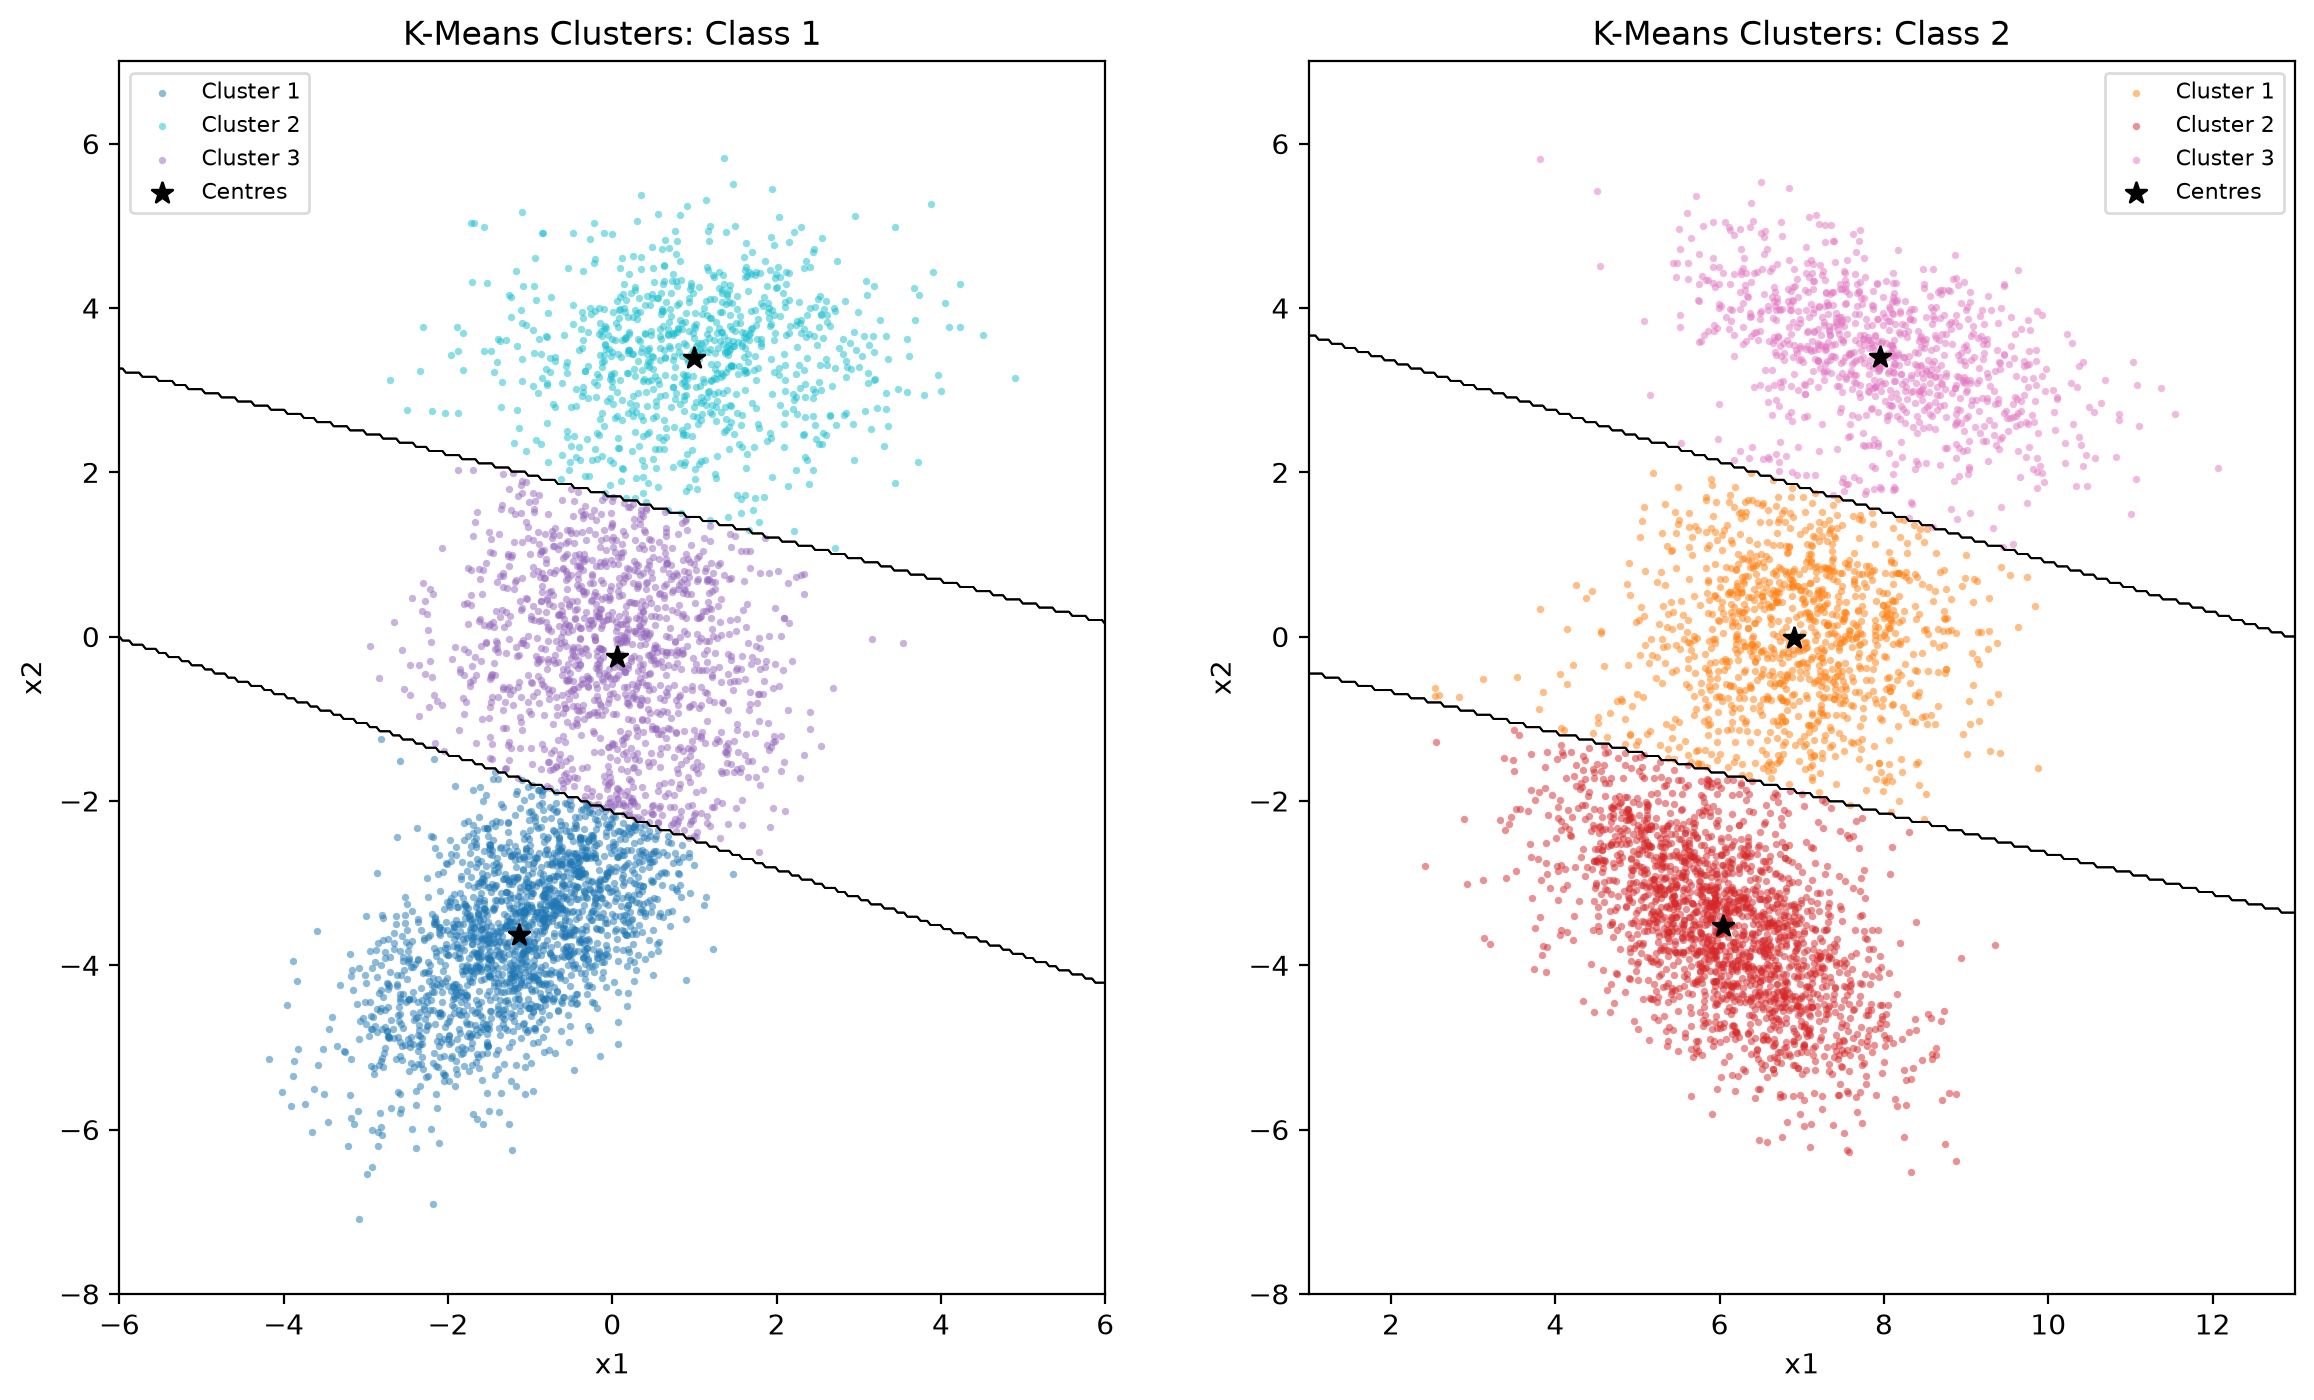
\includegraphics[width=0.96\textwidth]{cluster_boundaries.png}
\caption{Within-class K-means cluster boundaries and learned centres, using training data.}
\end{figure}

\section*{CLASSIFICATION OF TEST DATA}

Finally we also look at the decision boundary between the 2 Classes as well and along the way we would also look at the confusion matrix. So, Inorder to decide which class a particular point goes to, we would go calculate the distances between every learned centroid and assign it to the nearest centroids class.

\begin{figure}[H]
\centering
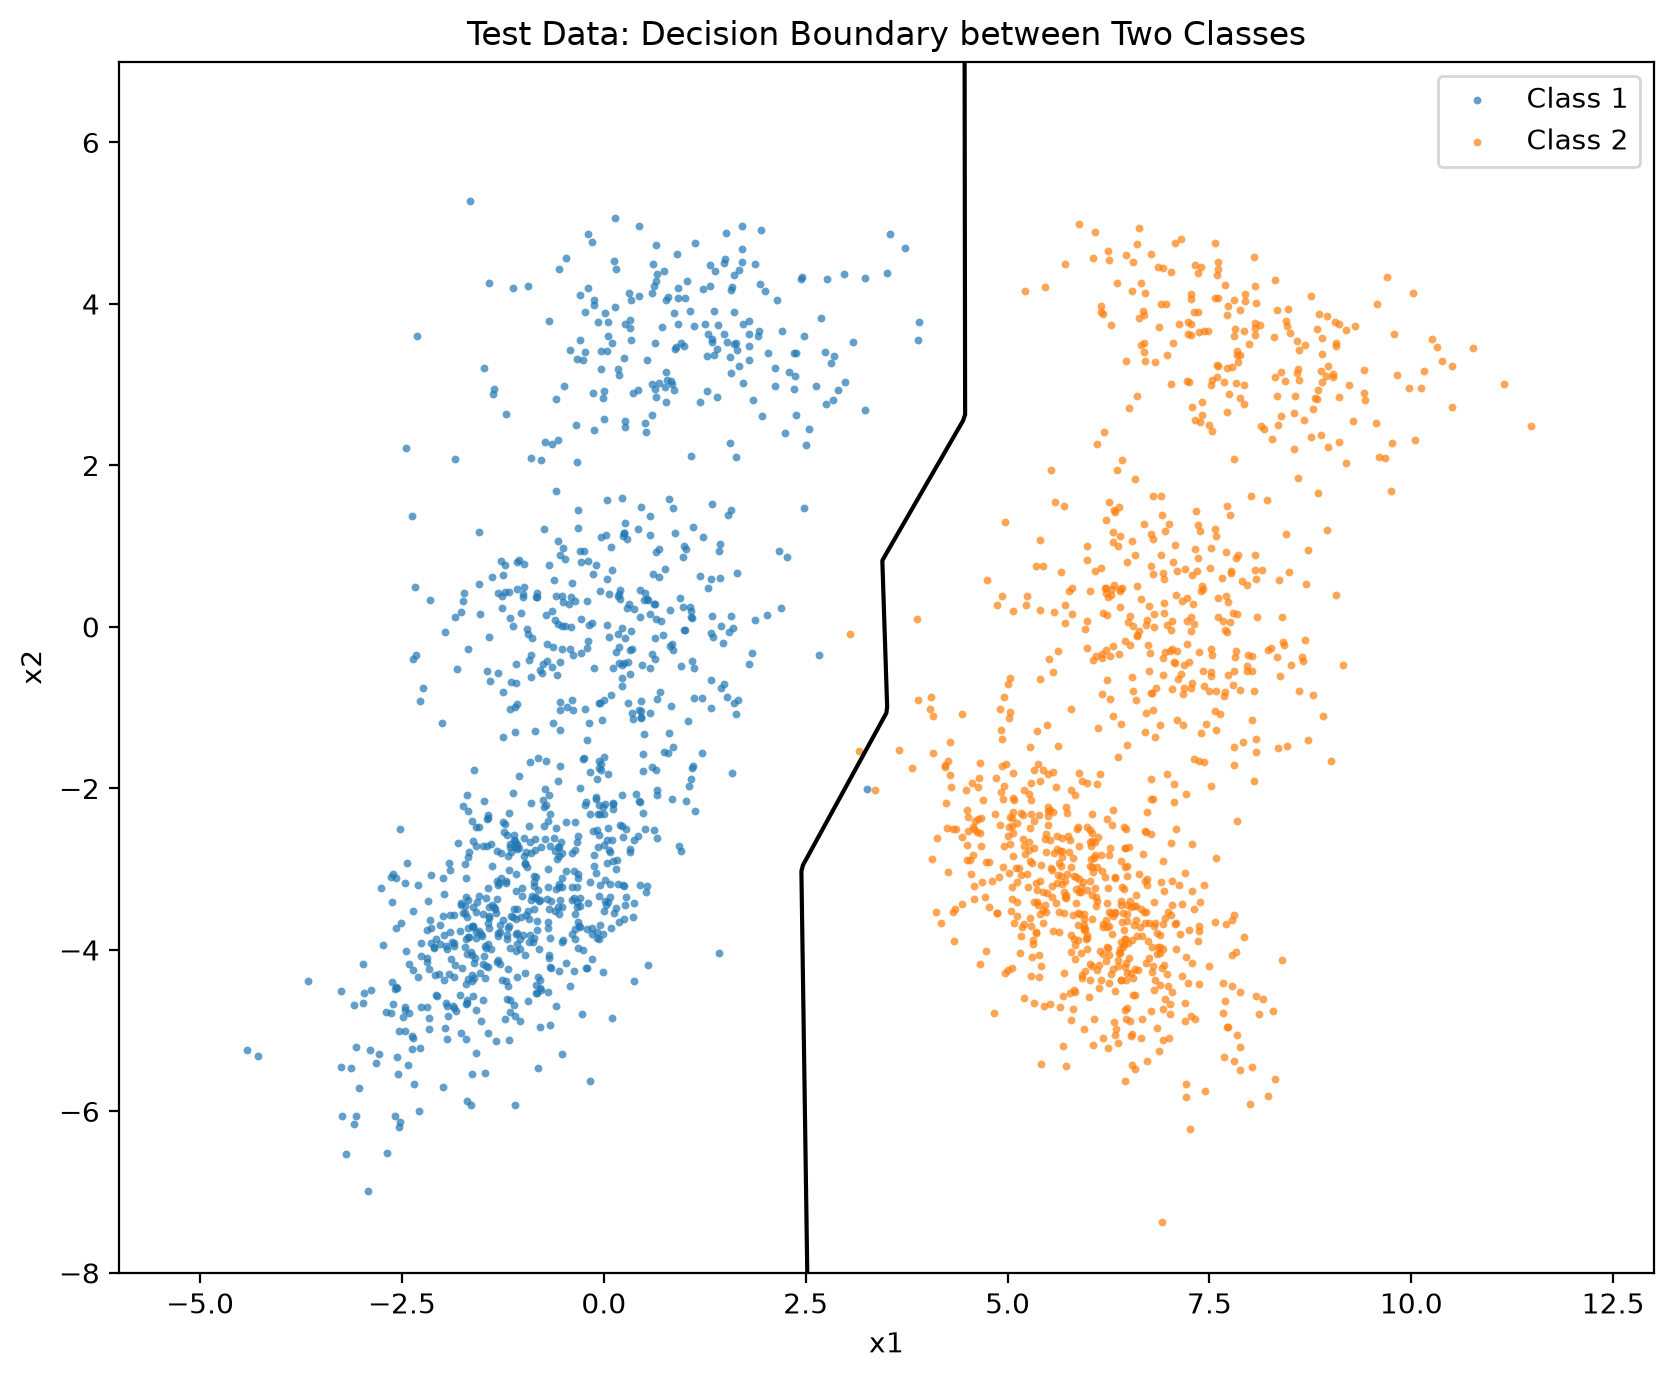
\includegraphics[width=0.70\textwidth]{class_boundary.png}
\caption{Held-out points coloured by true class, with the nearest-centre class decision boundary.}
\end{figure}

\section*{CLASSIFICATION RESULTS}
\begin{center}
\begin{tabular}{lcc}
\toprule
 & Predicted class 1 & Predicted class 2 \\
\midrule
True class 1 & 999 & 1 \\
True class 2 & 2 & 998 \\
\bottomrule
\end{tabular}
\end{center}
\textbf{Test accuracy: 99.85\%} \quad (1,997 correct out of 2,000).

Since, we had our data points for 2 classes well seperated there are only a very few misclassification as seen the figure.

\section*{INFERENCE}

The key takeaway from this assignment was to realize there can be many gaussians within a single class and we realized the importance of gaussian mixture models. Also, we understood the role of K-means (i.e.) to learn a few representations (centroids) and use them to classify new points.

\end{document}
